\section{A Practical Demonstration of Our Loss.}
%\vk{i don't think that the rest of this section belongs in the methods section; i would first make it less verbose, then i would move large parts of it to the experiments, and i would summarize here in 1-2 sentences} 

We experiment with how well-behaved our loss is on StackedMNIST~\cite{pacgan} which consists of 1000 uniformly-distributed modes. The network is a small ResNet~\cite{resnet2} for $G$ and $D$ without any normalization layers~\cite{bn,gn,ln,in}.
Through the use of a pretrained MNIST classifier, we can explicitly measure how many modes of $p_\mathcal{D}$ are recovered by $p_\theta$. Furthermore, we can estimate the reverse KL divergence between the fake and real samples $D_\text{KL}\left(p_\theta\parallel p_\mathcal{D} \right)$ via the KL divergence between the categorical distribution of $p_\theta$ and the true uniform distribution.
\begin{figure}[t]
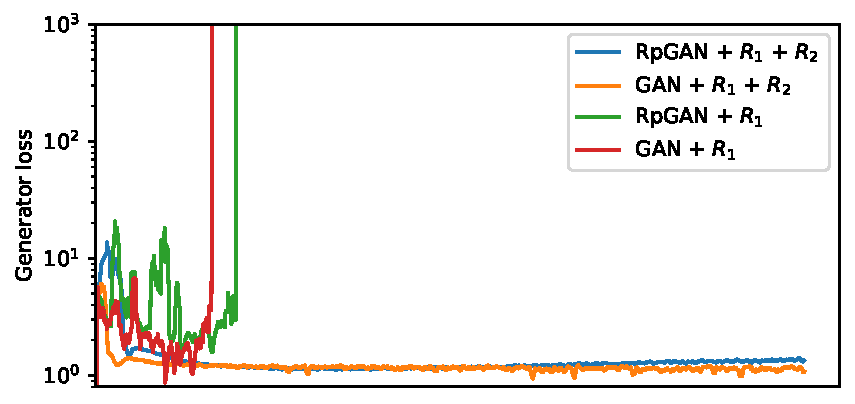
\includegraphics[width=1\linewidth]{figures/MNIST_loss.pdf}
\caption{Generator $G$ loss for different objectives over training. Regardless of which objective is used, training diverges with only $R_1$ and succeeded with both $R_1$ and $R_2$. Convergence failure with only $R_1$ was noted by Lee et al.~\cite{vitgan}.}
\label{fig:mnist_loss_curve}
\end{figure}

%For our initial experiments, we adopt a small ResNet~\cite{resnet2} architecture without any normalization layer~\cite{bn,gn,ln,in} for $G$ and $D$. 
A conventional GAN loss with $R_1$, as used by Mescheder et al.~\cite{r1} and the StyleGAN series~\cite{sg1, sg2, sg3}, diverges quickly (Fig.~\ref{fig:mnist_loss_curve}). Next, while theoretically sufficient for local convergence, RpGAN with only $R_1$ regularization is also unstable and diverges quickly\footnote{Varying $\gamma$ from 0.1 to 100 does not stabilize training.}. In each case, the gradient of $D$ on fake samples explodes when training diverges. With both $R_1$ and $R_2$, training becomes stable for both the classic GAN and RpGAN. Now stable, we can see that the classic GAN suffers from mode dropping, whereas RpGAN achieves full mode coverage (Table~\ref{tab:loss}) and reduces $D_\text{KL}$ from 0.9270 to 0.0781. As a point of contrast, StyleGAN~\cite{sg1,sg2,sg2ada,sg3} uses the minibatch standard deviation trick to reduce mode dropping, improving mode coverage from 857 to 881 on StackedMNIST and with barely any improvement on $D_\text{KL}$~\cite{pggan}.

%With training instability out of our way, we are ready to examine quantitatively how our new loss performs compared to existing work~\cite{r1,pggan,sg2}. While with $R_1$ and $R_2$ in conjunction training is successful for both the classic GAN~\cite{gan} and RpGAN~\cite{rgan}, we see in Table~\ref{tab:loss} that the classic GAN suffers from mode dropping. In contrast, RpGAN not only achieves full mode coverage, more notably, it drastically reduces $D_\text{KL}$ from 0.927 to 0.0781, indicating a considerably more faithful reconstruction of $p_\mathcal{D}$. 

% Instead of modifying the loss function, the StyleGAN family~\cite{sg1,sg2,sg2ada,sg3} relies on a trick called minibatch standard deviation~\cite{pggan} to combat mode dropping. It is shown in~\cite{pggan} that minibatch standard deviation can only slightly improve mode coverage from 857 to 881 on StackedMNIST and it shows barely any improvement on $D_\text{KL}$. 
% RpGAN in comparison improves mode coverage from 693 to 1000 and reduces $D_\text{KL}$ by one magnitude. 
%This shows that RpGAN is not only more principled against mode dropping in theory, but more effective in practice too. 
% We show in Section.\ref{sec:exp} that with architectural improvements in Section.\ref{sec:roadmap}, we can further improve $D_\text{KL}$ on StackedMNIST and even beat likelihood-based models. For the rest of this work, RpGAN $+ R_1+R_2$ will be our loss function.

% We start with RpGAN with only $R_1$ regularization since theoretically this is sufficient for local convergence. Contrary to our expectations, the training process utilizing this loss function exhibited significant instability and rapidly diverged. We experimented with various values of $\gamma$, ranging from 0.1 to 100; however, none succeeded in stabilizing the training. Furthermore, we explored integrating the conventional GAN loss combined with $R_1$, as commonly employed in the work of Mescheder et al.~\cite{r1} and the StyleGAN series~\cite{sg1, sg2, sg3}. Notably, this configuration led to even quicker divergence than the $R_1$ regularized RpGAN.
%To our surprise, training with this loss has been quite unstable and it diverges very quickly. We tried different $\gamma$ values ranging from 0.1 to 100 but none could prevent training from diverging. We also experiment with the combination of classic GAN and $R_1$, this is the widely adopted GAN loss in Mescheder~\etal~\cite{r1} and the StyleGAN family~\cite{sg1,sg2,sg3}, yet this loss diverges even faster than $R_1$ regularized RpGAN. 

% Upon closer inspection, we notice that the gradient of $D$ on fake samples explodes when training diverges. This motivates us to also apply $R_2$ regularization along with $R_1$, we see in Figure~\ref{fig:mnist_loss_curve} that with both $R_1$ and $R_2$, training becomes stable for both the classic GAN and RpGAN. 

\begin{table}[h]
\centering
    \begin{tabular}{ l rrr }
        \toprule
        Loss & \# modes$\uparrow$ & $D_\text{KL}$$\downarrow$ \\
        \midrule
        RpGAN $+ R_1+R_2$ & $\mathbf{1000}$ & $\mathbf{0.0781}$ \\
        GAN $+ R_1+R_2$ & $693$ & $0.9270$ \\
        RpGAN $+ R_1$ & Fail & Fail \\
        GAN $+ R_1$ & Fail & Fail \\
        \bottomrule
    \end{tabular}
    \caption{StackedMNIST~\cite{pacgan} result for each loss function. The maximum possible mode coverage is 1000. ``Fail'' indicates that training diverged early on.}
    \label{tab:loss}
\end{table}

$R_1$ alone is not sufficient for globally-convergent training. While a theoretical analysis of this is difficult, our small demonstration still provides insights into the assumptions of our convergence proof. 
In particular, the assumption that $(\theta,\psi)$ are sufficiently close to $(\theta^*,\psi^*)$ is highly unlikely early in training. In this scenario, if $D$ is sufficiently powerful, regularizing $D$ solely on real data is not likely to have much effect on $D$'s behavior on fake data and so training can fail due to an ill-behaved $D$ on fake data. 
% \vk{this is the key part that should be summarized in 1-2 sentences in this section: you find empirically and mathematically that both types of regularization are needed to make things work; then in the experiments section or in the appendix you provide results that show that it's the case}

Thus, the practical solution is to regularize $D$ on both real and fake data. The benefit of doing so can be viewed from the insight of Roth~\etal~\cite{r1r2}: that applying $R_1$ and $R_2$ in conjunction smooths both $p_\mathcal{D}$ and $p_\theta$ which makes learning easier than only smoothing $p_\mathcal{D}$. We also find empirically that with both $R_1$ and $R_2$ in place, $D$ tends to satisfy $\mathbb{E}_{x\sim p_\mathcal{D}}\left[\left\| \nabla_x D \right \|^2\right]\approx\mathbb{E}_{x\sim p_\theta}\left[\left\| \nabla_x D \right \|^2\right]$ even early in the training. Jolicoeur-Martineau~\etal~\cite{ganmmc} show that in this case $D$ becomes a maximum margin classifier---but if only one regularization term is applied, this does not hold.

% \vk{by the way, you will need a discussion of your regularization to other uses of this similar regularizer in the discussion or related work section}



\section{Experimental Findings from Config B.}
Violating \ref{item:convergent}, \ref{item:learning_rate}, or \ref{item:normalization} often leads to training failures.
%, contributing to the reputation that GANs as difficult to train. 
Gidel~\etal~\cite{ganmomentum} show that \emph{negative} momentum can improve GAN training dynamics. Since optimal negative momentum is another challenging hyperparameter, we do not use any momentum to avoid worsening GAN training dynamics. Studies~\cite{sg2,edm2} suggest normalization layers harm generative models. Batch normalization~\cite{bn} often cripples training due to dependencies across multiple samples, and is incompatible with $R_1$, $R_2$, or RpGAN that assume independent handling of each sample. Weaker data-independent normalizations~\cite{sg2,edm2} might help; we leave this for future work. Early GANs may succeed despite violating \ref{item:convergent} and \ref{item:normalization}, possibly constituting a full-rank solution~\cite{r1} to Eq.~\ref{eq:gan}.

Violations of \ref{item:resampling} or \ref{item:activation} do not significantly impair training stability but negatively affect sample quality. Improper transposed convolution can cause checkerboard artifacts, unresolved even with subpixel convolution~\cite{subpixel} or carefully tuned transposed convolution unless a low-pass filter is applied. Interpolation methods avoid this issue, varying from nearest neighbor~\cite{pggan} to Kaiser filters~\cite{sg3}. We use bilinear interpolation for simplicity. For activation functions, smooth approximations of (leaky) ReLU, such as Swish~\cite{swish}, GELU~\cite{gelu}, and SMU~\cite{smu}, worsen FID. PReLU~\cite{prelu} marginally improves FID but increases VRAM usage, so we use leaky ReLU.

All subsequent configurations adhere to \ref{item:convergent} through \ref{item:activation}. Violation of \ref{item:input} is acceptable as it pertains to the network backbone of StyleGAN2~\cite{sg2}, modernized in Config D and E.


\section{Network Architecture Details of Config D}
\vspace{-0.5ex}
Given i.\ref{item:i3}, i.\ref{item:i4}, and principles c), d), and e), we can replace the StyleGAN2 backbone with a modernized ResNet. We use a fully symmetric design for $G$ and $D$ with 25M parameters each, comparable to Config-A. The architecture is minimalist: each resolution stage has one transition layer and two residual blocks. The transition layer consists of bilinear resampling and an optional $1\times1$ conv for changing spatial size and feature map channels. The residual block includes five operations: Conv$1\times1\rightarrow$ Leaky ReLU $\rightarrow$ Conv$3\times3\rightarrow$ Leaky ReLU $\rightarrow$ Conv$1\times1$, with the final Conv$1\times1$ having no bias term. For the $4\times4$ resolution stage, the transition layer is replaced by a basis layer for $G$ and a classifier head for $D$. The basis layer, similar to StyleGAN~\cite{sg1,sg2}, uses $4\times4$ learnable feature maps modulated by $z$ via a linear layer. The classifier head uses a global $4\times4$ depthwise conv.~to remove spatial extent, followed by a linear layer to produce $D$'s output. We maintain the width ratio for each resolution stage as in Config A, making the stem width $3\times$ as wide due to the efficient $1\times1$ conv. The $3\times3$ conv in the residual block has a compression ratio of 4, following~\cite{resnet,resnet2}, making the bottleneck width $0.75\times$ as wide as Config A.
%Given i.3), i.4) and principles c), d), and e), we are now ready to replace the StyleGAN2 backbone with a modernized ResNet. We adopt a fully symmetric design for $G$ and $D$, and make the model size comparable to Config A, both $G$ and $D$ have approximately 25M parameters. We keep the architecture as minimalist as possible, for each resolution stage, we have one transition layer and two residual blocks. The transition layer consists of bilinear resampling and an optional $1\times1$ conv that allows us to change the spatial size and the number of channels of the feature maps. The residual block contains five consecutive operations on the residual branch: Conv$1\times1\rightarrow$ Leaky ReLU $\rightarrow$ Conv$3\times3\rightarrow$ Leaky ReLU $\rightarrow$ Conv$1\times1$, and the final Conv$1\times1$ has no bias term. For the $4\times4$ resolution stage, the transition layer is replaced by a basis layer for $G$ and a classifier head for $D$. The basis layer resembles the const input of StyleGAN~\cite{sg1,sg2} where a set of $4\times4$ learnable feature maps are modulated by $z$ via a linear layer. The classifier head first removes the spatial extent of the feature maps with a global $4\times4$ depthwise conv; the features are then fed to a linear layer to produce the output of $D$. We keep the width ratio for each resolution stage the same as Config A, and we are able to make the stem width $3\times$ as wide as Config A given the same model size thanks to the more efficient $1\times1$ conv. The compression ratio for the $3\times3$ conv in the residual block is set to 4 following~\cite{resnet,resnet2}, this makes the bottleneck width $0.75\times$ as wide as Config A.

% The lack of normalization necessitates more careful initialization for ResNet to avoid variance explosion. We apply fix-up initialization~\cite{fixup} to our modernized networks to remedy this. Concretely, we zero-initialize the last conv layer in each residual block, and scale down the initialization of the other two conv layers in the residual block by $L^{-0.25}$ where $L$ is the number of residual blocks in the network. We do not employ any other trick from fixup~\cite{fixup} such as applying excessive bias terms and the use of a scalar multiplier. The new network architecture and the initialization scheme allow us to raise the learning rate to $1\times10^{-4}$ without encountering training instability.
To avoid variance explosion due to the lack of normalization, we employ fix-up initialization~\cite{fixup} for our modernized networks. Specifically, we zero-initialize the last convolutional layer in each residual block and scale down the initialization of the other two convolutional layers in the block by $L^{-0.25}$, where $L$ is the number of residual blocks. We avoid other fix-up tricks, such as excessive bias terms and a learnable multiplier.

% We show that removing all these architectural modifications of the original StyleGAN mildly harms performance, but not as much as one might expect in~\ref{sub:arc-experiments}. Furthermore, removing some components actually benefits FID.


% \begin{figure}
%     \centering
%     \includegraphics[width=0.25\linewidth]{example-image-a}

%     \caption{Swirl Figure. We show our model matches performance on Gaussian toy example. \aaron{Are we still doing a toy example}]}
%     \label{fig:enter-label}
% \end{figure}

% \begin{figure}
%     \centering
%     \includegraphics[width=0.25\linewidth]{example-image-b}
%     \caption{k-NN decision barrier. Intuitive example}
%     \label{fig:enter-label}
% \end{figure}
\vspace{-1ex}
\section{Roadmap Insights}
\vspace{-0.5ex}
\begin{table}[t]
\resizebox{1\linewidth}{!}{
\begin{tabular}{ l r c c c } 
\toprule
   & \multicolumn{1}{l}{Configuration}  & FID$\downarrow$                    & G \#params              & D \#params               \\ 
\midrule
A  & \multicolumn{1}{l}{StyleGAN2}  & 7.516                  & 24.767M                  & 24.001M                   \\
\midrule
B  & \multicolumn{1}{l}{Stripped StyleGAN2}                                                                                                                                                                                                                                                                                                                                                                                                                 &                        &                          &                           \\ 
   & \begin{tabular}[c]{@{}r@{}}\textcolor{red}{- $z$ normalization}\\ \textcolor{red}{- Minibatch stddev}\\ \textcolor{red}{- Equalized learning rate}\textcolor{red}{}\\\textcolor{red}{- Mapping network}\\ \textcolor{red}{- Style injection}\\ \textcolor{red}{- Weight mod / demod}\\ \textcolor{red}{- Noise injection}\\ \textcolor{red}{- Mixing regularization}\\ \textcolor{red}{- Path length regularization}\\ \textcolor{red}{- Lazy regularization}\textcolor{blue}{}\end{tabular} & \multirow{2}{*}{12.46} & \multirow{2}{*}{18.890M} & \multirow{2}{*}{23.996M}  \\ 
\midrule
C  & \multicolumn{1}{l}{Well-behaved Loss}                       &                        &                          &                           \\ 
 & \textcolor[rgb]{0,0.502,0.502}{+ RpGAN loss}                                                                                                                                                                                                                                                                                                                                                                                                                   & 11.77                                           & \multirow{2}{*}{18.890M} & \multirow{2}{*}{23.996M}                           \\ 
   & \textcolor[rgb]{0,0.502,0.502}{+ $R_2$ gradient penalty}                                                                                                                                                                                                                                                                                                                                                                                                & \multirow{1}{*}{11.65} &                          &                           \\ 
\midrule
D  & \multicolumn{1}{l}{ConvNeXt-ify pt.~1}                                                                                                                                                                                                                                                                                                                                                                                                                 &                        &                          &                           \\ 
 & \textcolor[rgb]{0,0.502,0.502}{+ ResNet-ify G $\&$ D}                                                                                                                                                                                                                                                                                                                                                                                                   & 10.17                  & 23.400M                  & \multirow{2}{*}{23.282M}  \\
   & \textcolor{red}{- Output skips}                                                                                                                                                                                                                                                                                                                                                                                                                         & 9.950 & 23.378M &                           \\ 
\midrule
E  & \multicolumn{1}{l}{ConvNeXt-ify pt.~2}                              &                        &                          &                           \\
 & \textcolor[rgb]{0,0.502,0.502}{+ ResNeXt-ify G $\&$ D}                                                                                                                                                                                                                                                                                                                                                                                                  & 7.507                  & 23.188M                  & 23.091M                   \\ 
   & \textcolor[rgb]{0,0.502,0.502}{+ Inverted bottleneck}                                                                                                                                         & 7.045 & 23.058M & 23.010M  \\ 
\bottomrule
\end{tabular}
}
\vspace{-0.25cm}
\caption{Model configuration performance and size.} 
\label{tab:roadmap}
\vspace{-1ex}
\end{table}

As per Table~\ref{tab:roadmap}, Config A (vanilla StyleGAN2) achieves an FID of 7.52 using the official implementation on FFHQ-256. Config B with all tricks removed achieves an FID of 12.46---performance drops as expected. 
Config C, with a well-behaved loss, achieves an FID of 11.65. But, now training is sufficiently stable to improve the architecture.

Config D, which improves $G$ and $D$ based on the classic ResNet and ConvNeXt findings, achieves an FID of 9.95. The output skips of the StyleGAN2 generator are no longer useful given our new architecture; including them produces a worse FID of 10.17. Karras~\etal find that the benefit of output skips is mostly related to gradient magnitude dynamics~\cite{sg3}, and this has been addressed by our ResNet architecture. For StyleGAN2, Karras~\etal conclude that a ResNet architecture is harmful to $G$~\cite{sg2}, but this is not true in our case as their ResNet implementation is considerably different from ours: 1) Karras~\etal use one 3-3 residual block for each resolution stage, while we have a separate transition layer and two 1-3-1 residual blocks; 2) i.3) and i.4) are violated as they do not have a linear residual block~\cite{mobnet} and the transition layer is placed on the skip branch of the residual block rather than the stem; 3) the essential principle of ResNet~\cite{resnet}---identity mapping~\cite{resnet2}---is violated as Karras~\etal divide the output of the residual block by $\sqrt{2}$ to avoid variance explosion due to the absence of a proper initialization scheme.

For Config E, we conduct two experiments that ablate i.\ref{item:i1} (increased width with depthwise conv.) and i.\ref{item:i2} (an inverted bottleneck). We add GroupedConv and reduce the bottleneck compression ratio to two given the same model size. Each bottleneck is now 1.5$\times$ the width of Config A, and the FID drops to 7.51, surpassing the performance of StyleGAN2. By inverting the stem and the bottleneck dimensions to enhance the capacity of GroupedConv, our final model achieves an FID of 7.05, exceeding StyleGAN2.

\section{Experiments Details}
\begin{table}[]
\begin{tblr}{
  cell{2}{2} = {c},
  cell{2}{3} = {c},
  cell{3}{2} = {c},
  cell{3}{3} = {c},
  cell{4}{2} = {c},
  cell{4}{3} = {c},
  cell{5}{2} = {c},
  cell{5}{3} = {c},
  cell{6}{2} = {c},
  cell{6}{3} = {c},
  cell{7}{2} = {c},
  cell{7}{3} = {c},
  cell{8}{2} = {c},
  cell{8}{3} = {c},
  cell{9}{2} = {c},
  cell{9}{3} = {c},
  cell{10}{2} = {c},
  cell{10}{3} = {c},
  cell{11}{2} = {c},
  cell{11}{3} = {c},
  cell{12}{2} = {c},
  cell{12}{3} = {c},
  hline{2,12} = {1-3}{},
}
Model     & \# modes$\uparrow$ & $D_\text{KL}$$\downarrow$            &  \\
DCGAN~\cite{dcgan}     & 99            & 3.40\phantom{0}&  \\
VEEGAN~\cite{srivastava2017veegan}    & 150           & 2.95\phantom{0}&  \\
WGAN-GP~\cite{wgan-gp}& 959           & 0.73\phantom{0}&  \\
PacGAN~\cite{pacgan}    & 992           & 0.28\phantom{0}&  \\
StyleGAN2~\cite{sg2} & 940           & 0.42\phantom{0}&  \\
PresGAN~\cite{presgan}   & \textbf{1000} & 0.12\phantom{0}&  \\
Adv. DSM~\cite{advsm}  & \textbf{1000} & 1.49\phantom{0}&  \\
VAEBM~\cite{vaebm}     & \textbf{1000} & 0.087          &  \\
DDGAN~\cite{ddgan}     & \textbf{1000} & 0.071          &  \\
MEG~\cite{meg}       & \textbf{1000} & 0.031          &  \\
Ours---Config E     & \textbf{1000} & \textbf{0.029} &  
\end{tblr}
\caption{StackedMNIST 1000-mode coverage.}
\label{tab:stackedmnist}
\end{table}





\subsection{Mode recovery --- StackedMNIST\texorpdfstring{~\cite{metz2016unrolled}}{}} 
\vspace{-0.1cm}
We repeat the earlier experiment in 1000-mode convergence on StackedMNIST (unconditional generation), but this time with our updated architecture and with comparisons to SOTA GANs and likelihood-based methods (Tab.~\ref{tab:stackedmnist}, Fig.~\ref{fig:stacked-mnist}). 
One advantage brought up of likelihood-based models such as diffusion over GANs is that they achieve mode coverage~\cite{adm}. We find that most GANs struggle to find all modes. But, PresGAN~\cite{presgan}, DDGAN~\cite{ddgan} and our approach are successful. Further, our method outperforms all other tested GAN models in term of KL divergence.

\subsection{FID --- FFHQ-256\texorpdfstring{~\cite{sg1}}{} (Optimized)}
\vspace{-0.1cm}
We train Config E model until convergence and with optimized hyperparameters and training schedule on FFHQ at $256 \times 256$ (unconditional generation) (Tab.~\ref{tab:ffhq256}, Figs.~\ref{fig:ffhq-256-teaser} and~\ref{fig:ffhq-256}). The hyperparameters and schedule are listed in Appendix J. We outperform existing StyleGAN methods, plus four more recent diffusion-based methods. This particular dataset experimental setting is so common that many methods (not listed here) use the bCR~\cite{zhao2021improved} trick---this has only been shown to improve performance on FFHQ-256 (not even at different resolutions of FFHQ)~\cite{zhao2021improved, zhang2022styleswin}. We use no such tricks in our method.
% to achieve this performance.

\begin{figure}[h!]
    \newlength{\imgsize}
    \setlength{\imgsize}{0.10\linewidth} % Adjust this value to change the size of the images
    
    % New command to include images from a specific directory
    \newcommand{\qualitativeimg}[1]{%
        \includegraphics[width=\imgsize]{figures/qualitative/ffhq-256-000139623/image-#1.jpg}%
    }
    
    \setlength{\tabcolsep}{0pt} % Remove spacing between columns
    \renewcommand{\arraystretch}{0} % Remove spacing between rows
    
    \centering
    \begin{tabular}{cccccccc} % Eight columns
        \qualitativeimg{64} & \qualitativeimg{65} & \qualitativeimg{66} & \qualitativeimg{67} & \qualitativeimg{128} & \qualitativeimg{69} & \qualitativeimg{70} & \qualitativeimg{71} \\
        \qualitativeimg{72} & \qualitativeimg{73} & \qualitativeimg{74} & \qualitativeimg{75} & \qualitativeimg{76} & \qualitativeimg{77} & \qualitativeimg{78} & \qualitativeimg{79} \\
        \qualitativeimg{80} & \qualitativeimg{81} & \qualitativeimg{82} & \qualitativeimg{83} & \qualitativeimg{84} & \qualitativeimg{85} & \qualitativeimg{86} & \qualitativeimg{87} \\
        \qualitativeimg{88} & \qualitativeimg{89} & \qualitativeimg{90} & \qualitativeimg{91} & \qualitativeimg{92} & \qualitativeimg{93} & \qualitativeimg{94} & \qualitativeimg{95} \\
        \qualitativeimg{96} & \qualitativeimg{97} & \qualitativeimg{98} & \qualitativeimg{99} & \qualitativeimg{100} & \qualitativeimg{101} & \qualitativeimg{102} & \qualitativeimg{103} \\
        \qualitativeimg{104} & \qualitativeimg{105} & \qualitativeimg{106} & \qualitativeimg{107} & \qualitativeimg{108} & \qualitativeimg{109} & \qualitativeimg{110} & \qualitativeimg{111} \\
        \qualitativeimg{112} & \qualitativeimg{113} & \qualitativeimg{114} & \qualitativeimg{115} & \qualitativeimg{116} & \qualitativeimg{117} & \qualitativeimg{118} & \qualitativeimg{119} \\
        \qualitativeimg{120} & \qualitativeimg{121} & \qualitativeimg{122} & \qualitativeimg{123} & \qualitativeimg{124} & \qualitativeimg{125} & \qualitativeimg{126} & \qualitativeimg{127} \\
    \end{tabular}
    \caption{Qualitative examples of sample generation from our Config E on FFHQ-256.}
    \label{fig:ffhq-256-teaser}
\end{figure}


\subsection{FID --- CIFAR-10~\cite{krizhevsky2009learning}} \vspace{-0.1cm}
We train Config E model until convergence and with optimized hyperparameters and training schedule on CIFAR-10 (conditional generation) (Tab.~\ref{tab:cifar10}, Fig.~\ref{fig:cifar10}). Our method outperforms many other GANs by FID even though the model has relatively small capacity. For instance, StyleGAN-XL~\cite{sgxl} has 18\ M parameters in the generator and 125\ M parameters in the discriminator, while our model has a 40\ M parameters between the generator and discriminator combined (Fig.~\ref{fig:fid-50k-vs-params-cifar-10}). Compared to diffusion models like LDM or ADM, GAN inference is significantly cheaper as it requires only one network function evaluation compared to the tens or hundreds of network function evaluations for diffusion models without distillation. 

\begin{figure}[h]
    \centering
    % \includegraphics[width=\linewidth,clip,trim={0 0 0 2cm}]{figures/Scatterplot-FID-Parameters-CIFAR10.eps}
    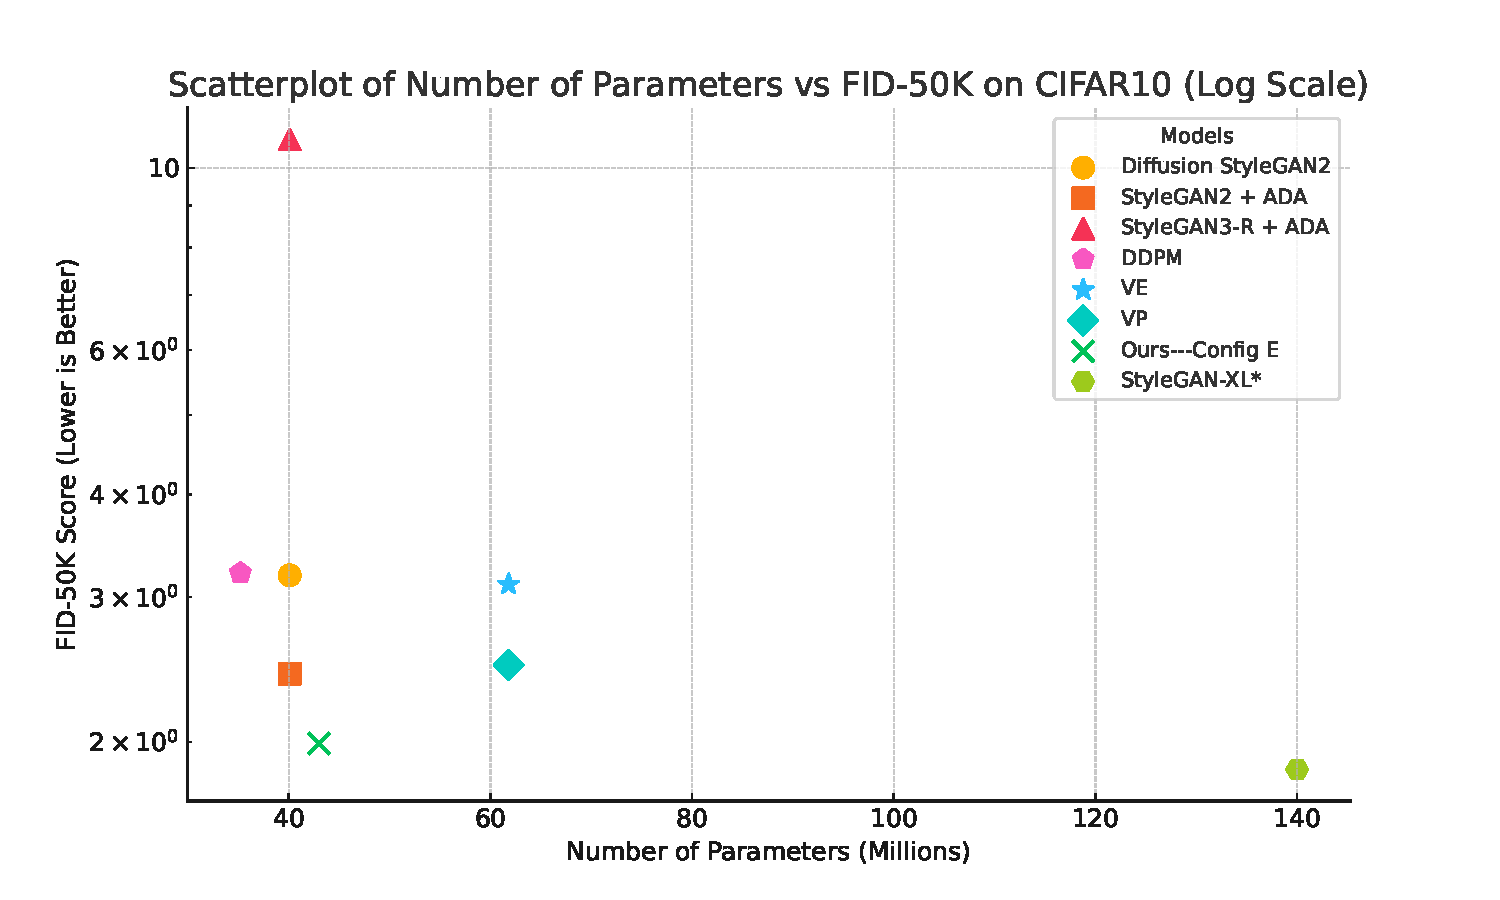
\includegraphics[width=\linewidth,clip,trim={0 0 0 2cm}]{figures/Scatterplot_FID_Parameters_CIFAR10_Log_Custom_Format.pdf}
    \caption{Number of parameters (millions) vs.~FID-50K (log scale) on CIFAR-10. Lower is better.}
    \label{fig:fid-50k-vs-params-cifar-10}
\end{figure}

Many state-of-the-art GANs are derived from Projected GAN~\cite{sauer2021projected}, including StyleGAN-XL~\cite{sgxl} and the concurrent work of StyleSAN-XL~\cite{takida2024san}. These methods use a pre-trained ImageNet classifier in the discriminator. Prior work has shown that a pre-trained ImageNet discriminator can leak ImageNet features into the model~\cite{kynkaanniemi2022role}, causing the model to perform better when evaluating on FID since it relies on a pre-trained ImageNet classifier for the loss. But, this does not improve results in perceptual studies~\cite{kynkaanniemi2022role}. Our model produces its low FID without any ImageNet pre-training.

\subsection{FID --- ImageNet-32~\cite{chrabaszcz2017downsampled}}

We train Config E model until convergence and with optimized hyperparameters and training schedule on ImageNet-32 (conditional generation). We compare against recent GAN models and recent diffusion models in Table~\ref{tab:imagenet32}.
We adjust the number of parameters in the generator of our model to match StyleGAN-XL~\cite{sgxl}'s generator (84 million parameters). Specifically, we make the model significantly wider to match. Our method achieves comparable FID despite using a 60\% smaller discriminator (Tab.~\ref{tab:imagenet32}) and despite not using a pre-trained ImageNet classifier.



\section{Discussion and Limitations}

We have shown that a simplication of GANs is possible for image generation tasks, built upon a more stable RpGAN$+ R_1 + R_2$ objective with mathematically-demonstrated convergence properties that still provides diverse output. This stability is what lets us re-engineer a modern network architecture without the tricks of previous methods, producing the \modelName model with competitive FID on the common datasets of Stacked-MNIST, FFHQ, CIFAR-10, and ImageNet-32 as an empirical demonstration of the mathematical benefits.

The focus of our work is to elucidate the essential components of a minimum GAN for image generation. 
As such, we prioritize simplicity over functionality---we do not claim to beat the performance of every existing model on every dataset or task; merely to provide a new simple baseline that converges easily.
While this makes our model an ideal backbone for future GANs, it also means that it is not suitable to apply our model directly to downstream applications such as image editing or controllable generation, as our model lacks dedicated features for easy image inversion or disentangled image synthesis. 
For instance, we remove style injection functionality from StyleGAN even though this has a clear use.
We also omitted common techniques that have been shown in previous literature to improve FID considerably. 
Examples include some form of adaptive normalization modulated by the latent code~\cite{adm,edm,sg1,zhang2022styleswin,dit}, and using multiheaded self attention at lower resolution stages~\cite{adm,edm,edm2}. 
We aim to explore these techniques in a subsequent study. 

Further, our work is limited in its evaluation of the scalability of \modelName models. While they show promising results on $32\times32$ ImageNet, we are yet to verify the scalability on higher resolution ImageNet data or large-scale text to image generation tasks.

Finally, as a method that can improve the quality of generative models, it would be amiss not to mention that generative models---especially of people---can cause direct harm (e.g., through personalized deep fakes) and societal harm through the spread of disinformation (e.g., fake influencers). 

\clearpage
\section{Local convergence}
Following~\cite{r1}, GAN training can be formulated as a dynamical system where the update operator is given by $F_h(\theta,\psi)=(\theta,\psi)+hv(\theta,\psi)$. $h$ is the learning rate and $v$ denotes the gradient vector field:
\begin{equation}
v(\theta,\psi)=\begin{pmatrix}
 -\nabla_\theta\mathcal{L}(\theta,\psi) \\
 \nabla_\psi\mathcal{L}(\theta,\psi)
\end{pmatrix}
\end{equation}
Mescheder et al.~\cite{gannum} showed that local convergence near $(\theta^*,\psi^*)$ can be analyzed by examining the spectrum of the Jacobian $\textbf{J}_{F_h}$ at the equilibrium: if the Jacobian has eigenvalues with absolute value bigger than 1, then training does not converge. On the other hand, if all eigenvalues have absolute value smaller than 1, then training will converge to $(\theta^*,\psi^*)$ at a linear rate. If all eigenvalues have absolute value equal to 1, the convergence behavior is undetermined.

Given some calculations~\cite{r1}, we can show that the eigenvalues of the Jacobian of the update operator $\lambda_{\textbf{J}_{F_h}}$ can be determined by $\lambda_{\textbf{J}_v}$:
\begin{equation}
\lambda_{\textbf{J}_{F_h}}=1+h\lambda_{\textbf{J}_v}\ .
\end{equation}
That is, given small enough $h$~\cite{r1}, the training dynamics can instead be examined using $\lambda_{\textbf{J}_v}$,~\ie, the eigenvalues of the Jacobian of the gradient vector field. If all $\lambda_{\textbf{J}_v}$ have a negative real part, the training will locally converge to $(\theta^*,\psi^*)$ at a linear rate. On the other hand, if some $\lambda_{\textbf{J}_v}$ have a positive real part, the training is not convergent. If all $\lambda_{\textbf{J}_v}$ have a zero real part, the convergence behavior is inconclusive.

\section{DiracRpGAN: A demonstration of non-convergence}
\paragraph{Summary.} To obtain DiracRpGAN, we apply Eq.~\ref{eq:rpgan} to the DiracGAN~\cite{r1} problem setting. After simplification, DiracRpGAN and DiracGAN are different only by a constant. They have the same gradient vector field, therefore all proofs are identical to Mescheder~\etal~\cite{r1}.

\paragraph{Definition B.1.} \emph{The DiracRpGAN consists of a (univariate) generator distribution $p_{\theta} = \delta_{\theta}$ and a linear discriminator $D_{\psi}(x) = \psi \cdot x$. The true data distribution $p_{\mathcal{D}}$ is given by a Dirac distribution concentrated at 0.}

In this setup, the RpGAN training objective is given by:
\begin{equation}
\label{eq:diracrpgan}
    \mathcal{L}(\theta, \psi) = f(\psi \theta)\ .
\end{equation}
We can now show analytically that DiracRpGAN does not converge without regularzation.

\paragraph{Lemma B.2.} \emph{The unique equilibrium point of the training objective in Eq.~\ref{eq:diracrpgan} is given by $\theta = \psi = 0$. Moreover, the Jacobian of the gradient vector field at the equilibrium point has the two eigenvalues $\pm f'(0)i$ which are both on the imaginary axis.}

The gradient vector field $v$ of Eq.~\ref{eq:diracrpgan} is given by:
\begin{equation}
    v(\theta, \psi) =
    \begin{pmatrix}
    -\nabla_{\theta} \mathcal{L}(\theta, \psi) \\
    \nabla_{\psi} \mathcal{L}(\theta, \psi)
    \end{pmatrix} =
    \begin{pmatrix}
    -\psi f'(\psi \theta) \\
    \theta f'(\psi \theta)
    \end{pmatrix}
\end{equation}
and the Jacobian of $v$:
\begin{equation}
    \textbf{J}_v =
    \begin{pmatrix}
    -\psi^2 f''(\psi\theta) & -f'(\psi\theta) - \psi\theta f''(\psi\theta) \\
    f'(\psi\theta) + \psi\theta f''(\psi\theta) & \theta^2 f''(\psi\theta)
    \end{pmatrix}
\end{equation}
Evaluating $\textbf{J}_v$ at the equilibrium point $\theta = \psi = 0$ gives us:
\begin{equation}
    \textbf{J}_v \biggr\rvert_{(0,0)} =
    \begin{pmatrix}
    0 & -f'(0) \\
    f'(0) & 0
    \end{pmatrix}
\end{equation}
Therefore, the eigenvalues of $\textbf{J}_v$ are $\lambda_{1/2} = \pm f'(0) i$, both of which have a real part of 0. Thus, the convergence of DiracRpGAN is inconclusive and further analysis is required.

\paragraph{Lemma B.3.} \emph{The integral curves of the gradient vector field $v(\theta, \psi)$ do not converge to the equilibrium point. More specifically, every integral curve $(\theta(t), \psi(t))$ of the gradient vector field $v(\theta, \psi)$ satisfies $\theta(t)^2 + \psi(t)^2 = const$ for all $t \in [0, \infty)$.}

Let $R(\theta, \psi) = \frac{1}{2} (\theta^2 + \psi^2)$, then:
\begin{align}
    & \frac{\mathrm{d}}{\mathrm{d}t} R(\theta(t), \psi(t)) \nonumber \\
    &= -\theta(t) \psi(t) f'(\theta(t) \psi(t)) + \psi(t) \theta(t) f'(\theta(t) \psi(t)) \nonumber \\
    &= 0\ .
\end{align}
We see that the distance between $(\theta, \psi)$ and the equilibrium point $(0,0)$ stays constant. Therefore, training runs in circles and never converges.

Next, we investigate the convergence behavior of DiracRpGAN with regularization. For DiracRpGAN, both $R_1$ and $R_2$ can be reduced to the following form:
\begin{equation}
    R(\psi) = \frac{\gamma}{2} \psi^2
\end{equation}

\paragraph{Lemma B.4.} \emph{The eigenvalues of the Jacobian of the gradient vector field for the gradient-regularized DiracRpGAN at the equilibrium point are given by
\begin{equation}
\label{eq:ev}
    \lambda_{1/2} = -\frac{\gamma}{2} \pm \sqrt{\frac{\gamma^2}{4}-f'(0)}
\end{equation}
In particular, for $\gamma > 0$ all eigenvalues have a negative real part. Hence, gradient descent is locally convergent for small enough learning rates.}

With regularization, the gradient vector field becomes
\begin{equation}
    \Tilde{v} (\theta, \psi) =
    \begin{pmatrix}
        -\psi f'(\psi\theta) \\
        \theta f'(\psi\theta) - \gamma\psi
    \end{pmatrix}
\end{equation}
the Jacobian of $\Tilde{v}$ is then given by
\begin{equation}
    \textbf{J}_{\Tilde{v}} =
    \begin{pmatrix}
    -\psi^2 f''(\psi\theta) & -f'(\psi\theta) - \psi\theta f''(\psi\theta) \\
    f'(\psi\theta) + \psi\theta f''(\psi\theta) & \theta^2 f''(\psi\theta) - \gamma
    \end{pmatrix}
\end{equation}
evaluating the Jacobian at $\theta = \psi = 0$ yields
\begin{equation}
    \textbf{J}_{\Tilde{v}} \biggr\rvert_{(0, 0)} =
    \begin{pmatrix}
        0 & -f'(0) \\
        f'(0) & -\gamma
    \end{pmatrix}
\end{equation}
given some calculations, we arrive at Eq.\ref{eq:ev}.

\section{General Convergence Results}
\paragraph{Summary.} The proofs are largely the same as Mescheder~\etal~\cite{r1}. We use the same proving techniques, and only slightly modify the assumptions and proof details to adapt Mescheder~\etal's effort to RpGAN. Like in~\cite{r1}, our proofs do not rely on unrealistic assumptions such as $\supp p_\mathcal{D}=\supp p_\theta$.

\subsection{Assumptions}
We closely follow~\cite{r1} but modify the assumptions wherever necessary to tailor the proofs for RpGAN. Like in~\cite{r1}, we also consider the realizable case where there exists $\theta$ such that $G_\theta$ produces the true data distribution.

\paragraph{Assumption~\upperRomannumeral{1}.}
\label{a:1}
\emph{We have $p_{\theta^*}=p_\mathcal{D}$, and $D_{\psi^*}=C$ in some local neighborhood of $\supp p_\mathcal{D}$, where $C$ is some arbitrary constant.}

\noindent Since RpGAN is defined on critic difference rather than raw logits, we no longer require $D_{\psi^*}$ to produce 0 on $\supp p_\mathcal{D}$, instead any constant $C$ would suffice.

\paragraph{Assumption~\upperRomannumeral{2}.}
\label{a:2}
\emph{We have $f^\prime(0)\neq0$ and $f^{\prime\prime}(0)<0$.}

\noindent This assumption is the same as in~\cite{r1}. The choice $f(t) = -\log(1+e^{-t})$ adopted in the main text satisfies this assumption.

As discussed in~\cite{r1}, there generally is not a single equilibrium point $(\theta^*,\psi^*)$, but a submanifold of equivalent equilibria corresponding to different parameterizations of the same function. It is therefore necessary to represent the equilibrium as \emph{reparameterization manifolds} $\mathcal{M}_G$ and $\mathcal{M}_D$. We modify the reparameterization $h$ as follows:
\begin{equation}
\label{eq:h}
h(\psi)=\mathbb{E}_{\substack{x\sim p_\mathcal{D}\\y\sim p_\mathcal{D}}}\left[\left | D_\psi(x)-D_\psi(y)\right |^2   +  \left \| \nabla_x D_\psi(x) \right \|^2\right]
\end{equation}
to account for the fact that $D_{\psi^*}$ is now allowed to have any constant value on $\supp p_\mathcal{D}$. The \emph{reparameterization manifolds} are then given by:
\begin{align}
&\mathcal{M}_G=\{\theta\ \rvert\ p_\theta=p_\mathcal{D}\} \\
&\mathcal{M}_D=\{\psi\ \rvert\ h(\psi)=0 \}
\end{align}
We assume the same regularity properties as in~\cite{r1} for $\mathcal{M}_G$ and $\mathcal{M}_D$ near the equilibrium. To state these assumptions, we need:
\begin{equation}
g(\theta)=\mathbb{E}_{x\sim p_\theta}\left[\nabla_\psi D_\psi\rvert_{\psi=\psi^*}\right]
\end{equation}
which leads to:
\paragraph{Assumption~\upperRomannumeral{3}.}
\label{a:3}
\emph{There are $\epsilon$-balls $B_\epsilon(\theta^*)$ and $B_\epsilon(\psi^*)$ around $\theta^*$ and $\psi^*$ so that $\mathcal{M}_G\ \cap\ B_\epsilon(\theta^*)$ and $\mathcal{M}_D\ \cap\ B_\epsilon(\psi^*)$ define $\mathcal{C}^1$-manifolds. Moreover, the following holds}:
\begin{enumerate}[label=(\roman*)]
\item \emph{if $v\in\mathbb{R}^n$ is not in $\mathcal{T}_{\psi^*}\mathcal{M}_D$, then $\partial_v^2h(\psi^*)\neq0$}.
\item \emph{if $w\in\mathbb{R}^m$ is not in $\mathcal{T}_{\theta^*}\mathcal{M}_G$, then $\partial_wg(\theta^*)\neq0$}.
\end{enumerate}

These two conditions have exactly the same meanings as in~\cite{r1}: the first condition indicates the geometry of $\mathcal{M}_D$ can be locally described by the second derivative of $h$. The second condition implies that $D$ is strong enough that it can detect any deviation from the equilibrium generator distribution. This is the only assumption we have about the expressiveness of $D$.

\subsection{Convergence}
We can now show the general convergence result for gradient penalized RpGAN, consider the gradient vector field with either $R_1$ or $R_2$ regularization:
\begin{equation}
\label{eq:vreg}
\tilde{v}_i(\theta,\psi)=\begin{pmatrix}
-\nabla_\theta\mathcal{L}(\theta,\psi)\\ 
\nabla_\psi\mathcal{L}(\theta,\psi)-\nabla_\psi R_i(\theta,\psi)
\end{pmatrix}
\end{equation}
note that the convergence result can also be trivially extended to the case where both $R_1$ and $R_2$ are applied. We omit the proof for this case as it is redundant once the convergence with either regularization is proven.

\paragraph{Theorem.} \emph{Assume Assumption~\upperRomannumeral{1},~\upperRomannumeral{2} and~~\upperRomannumeral{3} hold for $(\theta^*,\psi^*)$. For small enough learning rates, gradient descent for $\tilde{v}_1$ and $\tilde{v}_2$ are both convergent to $\mathcal{M}_G\times\mathcal{M}_D$ in a neighborhood of $(\theta^*,\psi^*)$. Moreover, the rate of convergence is at least linear}.

We extend the convergence proof by Mescheder~\etal~\cite{r1} to our setting. We first prove lemmas necessary to our main proof.

\paragraph{Lemma C.2.1.} \emph{Assume $J\in\mathbb{R}^{(n+m)\times(n+m)}$ is of the following form}:
\begin{equation}
J=\begin{pmatrix}
0 & -B^\top\\ 
B & -Q
\end{pmatrix}
\end{equation}
\emph{where $Q\in\mathbb{R}^{m\times m}$ is a symmetric positive definite matrix and $B\in\mathbb{R}^{m\times n}$ has full column rank. Then all eigenvalues $\lambda$ of $J$ satisfy $\Re(\lambda)< 0$}.

\emph{Proof.} See Mescheder~\etal~\cite{r1}, Theorem A.7.

\paragraph{Lemma C.2.2.} \emph{The gradient of $\mathcal{L}(\theta,\psi)$~\wrt $\theta$ and $\psi$ are given by}:
\begin{align}
\nabla_\theta\mathcal{L}(\theta,\psi)=\mathbb{E}_{\substack{z\sim p_z\\x\sim p_\mathcal{D}}}[f^\prime(D_\psi(G_\theta(z))-D_\psi(x)) \nonumber \\ 
\left[\nabla_\theta G_\theta(z)\right]^\top\nabla_xD_\psi(G_\theta(z))] \\
\label{grad_psi}
\nabla_\psi\mathcal{L}(\theta,\psi)=\mathbb{E}_{\substack{z\sim p_z\\x\sim p_\mathcal{D}}}[f^\prime(D_\psi(G_\theta(z))-D_\psi(x)) \nonumber \\
(\nabla_\psi D_\psi(G_\theta(z))-\nabla_\psi D_\psi(x))]
\end{align}
\emph{Proof.} This is just the chain rule.

\paragraph{Lemma C.2.3.} \emph{Assume that $(\theta^*,\psi^*)$ satisfies Assumption~\upperRomannumeral{1}. The Jacobian of the gradient vector field $v(\theta,\psi)$ at $(\theta^*,\psi^*)$ is then}
\begin{equation}
\textbf{J}_v\biggr\rvert_{(\theta^*,\psi^*)}=\begin{pmatrix}
0 & -K^\top_{DG}\\ 
K_{DG} & K_{DD}
\end{pmatrix}
\end{equation}
\emph{the terms $K_{DD}$ and $K_{DG}$ are given by}
\begin{align}
\label{kdd}
K_{DD}=f^{\prime\prime}(0)\mathbb{E}_{\substack{x\sim p_\mathcal{D}\\y\sim p_\mathcal{D}}}[(\nabla_\psi D_{\psi^*}(x)-\nabla_\psi D_{\psi^*}(y)) \nonumber \\
(\nabla_\psi D_{\psi^*}(x)-\nabla_\psi D_{\psi^*}(y))^\top] \\
\label{kdg}
K_{DG}=f^\prime(0)\nabla_\theta\mathbb{E}_{x\sim p_\theta}[\nabla_\psi D_{\psi^*}(x)]\ \rvert_{\theta=\theta^*}
\end{align}

\emph{Proof.} Note that
\begin{equation}
\textbf{J}_v\biggr\rvert_{(\theta^*,\psi^*)}=\begin{pmatrix}
-\nabla^2_\theta\mathcal{L}(\theta^*,\psi^*) & -\nabla^2_{\theta,\psi}\mathcal{L}(\theta^*,\psi^*) \\ 
\nabla^2_{\theta,\psi}\mathcal{L}(\theta^*,\psi^*) & \nabla^2_\psi\mathcal{L}(\theta^*,\psi^*)
\end{pmatrix}
\end{equation}
By Assumption~\upperRomannumeral{1}, $D_{\psi^*}=C$ in some neighborhood of $\supp p_\mathcal{D}$. Therefore we also have $\nabla_x D_{\psi^*}=0$ and $\nabla^2_x D_{\psi^*}=0$ for $x\in\supp p_\mathcal{D}$. Using these two conditions, we see that $\nabla^2_\theta\mathcal{L}(\theta^*,\psi^*)=0$.

To see Eq.\ref{kdd} and Eq.\ref{kdg}, simply take the derivatives of Eq.\ref{grad_psi} and evaluate at $(\theta^*,\psi^*)$.

\paragraph{Lemma C.2.4.} \emph{The gradient $\nabla_\psi R_i(\theta,\psi)$ of the regularization terms $R_i$, $i\in\{1,2\}$,~\wrt $\psi$ are}
\begin{align}
&\nabla_\psi R_1(\theta,\psi)=\gamma\mathbb{E}_{x\sim p_\mathcal{D}}[\nabla_{\psi,x}D_\psi\nabla_xD_\psi] \\
&\nabla_\psi R_2(\theta,\psi)=\gamma\mathbb{E}_{x\sim p_\theta}[\nabla_{\psi,x}D_\psi\nabla_xD_\psi]
\end{align}

\emph{Proof.} See Mescheder~\etal~\cite{r1}, Lemma D.3.

\paragraph{Lemma C.2.5.} \emph{The second derivatives $\nabla^2_\psi R_i(\theta^*,\psi^*)$ of the regularization terms $R_i$, $i\in\{1,2\}$,~\wrt $\psi$ at $(\theta^*,\psi^*)$ are both given by}
\begin{equation}
L_{DD}=\gamma\mathbb{E}_{x\sim p_\mathcal{D}}[AA^\top]
\end{equation}
\emph{where $A=\nabla_{\psi,x}D_{\psi^*}$. Moreover, both regularization terms satisfy $\nabla_{\theta,\psi}R_i(\theta^*,\psi^*)=0$.}

\emph{Proof.} See Mescheder~\etal~\cite{r1}, Lemma D.4.

Given Lemma C.2.3, Lemma C.2.5 and Eq.\ref{eq:vreg}, we can now show that the Jacobian of the regularized gradient field at the equilibrium point is given by
\begin{equation}
\textbf{J}_{\tilde{v}}\biggr\vert_{(\theta^*,\psi^*)}=\begin{pmatrix}
0 & -K_{DG}^\top\\ 
K_{DG} & M_{DD}
\end{pmatrix}
\end{equation}
where $M_{DD}=K_{DD}-L_{DD}$. To prove our main theorem, we need to examine $\textbf{J}_{\tilde{v}}$ when restricting it to the space orthogonal to $\mathcal{T}_{(\theta^*,\psi^*)}\mathcal{M}_G\times\mathcal{M}_D$.

\paragraph{Lemma C.2.6.} \emph{Assume Assumptions~\upperRomannumeral{2} and~\upperRomannumeral{3} hold. If $v\neq0$ is not in $\mathcal{T}_{\psi^*}\mathcal{M}_D$, then $v^\top M_{DD}v<0$.}

\emph{Proof.} By Lemma C.2.3 and Lemma C.2.5, we have
\begin{align}
\resizebox{0.42\textwidth}{!}{$
v^\top K_{DD}v=f^{\prime\prime}(0)\mathbb{E}_{\substack{x\sim p_\mathcal{D}\\y\sim p_\mathcal{D}}}\left[((\nabla_\psi D_{\psi^*}(x)-\nabla_\psi D_{\psi^*}(y))^\top v)^2\right]
$}
\end{align}
\begin{align}
v^\top L_{DD}v=\gamma\mathbb{E}_{x\sim p_\mathcal{D}}\left[\left\|Av\right \|^2\right]
\end{align}
By Assumption~\upperRomannumeral{2}, we have $f^{\prime\prime}(0)<0$. Therefore $v^\top M_{DD}v \leq 0$. Suppose $v^\top M_{DD}v=0$, this implies
\begin{equation}
(\nabla_\psi D_{\psi^*}(x)-\nabla_\psi D_{\psi^*}(y))^\top v=0\ \ \ \ \text{and}\ \ \ \ Av=0
\end{equation}
for all $(x,y)\in\supp\ p_\mathcal{D}\times\supp\ p_\mathcal{D}$. Recall the definition of $h(\psi)$ from Eq.\ref{eq:h}. Using the fact that $D_{\psi^*}=C$ and $\nabla_x D_{\psi^*}=0$ for $x\in\supp\ p_\mathcal{D}$, we see that the Hessian of $h(\psi)$ at $\psi^*$ is
\begin{align}
\nabla^2_\psi h(\psi^*)=2\mathbb{E}_{\substack{x\sim p_\mathcal{D}\\y\sim p_\mathcal{D}}}[(\nabla_\psi D_{\psi^*}(x)-\nabla_\psi D_{\psi^*}(y)) \nonumber \\
(\nabla_\psi D_{\psi^*}(x)-\nabla_\psi D_{\psi^*}(y))^\top+AA^\top]
\end{align}
The second directional derivative $\partial^2_v h(\psi)$ is therefore
\begin{align}
&\ \ \ \ \partial^2_v h(\psi) \nonumber \\
&=2\mathbb{E}_{\substack{x\sim p_\mathcal{D}\\y\sim p_\mathcal{D}}}\left[\left| (\nabla_\psi D_{\psi^*}(x)-\nabla_\psi D_{\psi^*}(y))^\top v\right|^2 + \left\|Av\right\|^2\right] \nonumber \\
&=0
\end{align}
By Assumption~\upperRomannumeral{3}, this can only hold if $v\in\mathcal{T}_{\psi^*}\mathcal{M}_D$.

\paragraph{Lemma C.2.7.} \emph{Assume Assumption~\upperRomannumeral{3} holds. If $w\neq0$ is not in $\mathcal{T}_{\theta^*}\mathcal{M}_G$, then $K_{DG}w\neq0$.}

\emph{Proof.} See Mescheder~\etal~\cite{r1}, Lemma D.6.

\emph{Proof for the main theorem.} Given previous lemmas, by choosing local coordinates $\theta(\alpha,\gamma_G)$ and $\psi(\beta,\gamma_D)$ for $\mathcal{M}_G$ and $\mathcal{M}_D$ such that $\theta^*=0$, $\psi^*=0$ as well as
\begin{align}
\mathcal{M}_G=\mathcal{T}_{\theta^*}\mathcal{M}_G=\{0\}^k\times\mathbb{R}^{n-k} \\
\mathcal{M}_D=\mathcal{T}_{\psi^*}\mathcal{M}_D=\{0\}^l\times\mathbb{R}^{m-l}
\end{align}
our proof is \emph{exactly} the same as Mescheder~\etal~\cite{r1}, Theorem 4.1.

\newpage
\section{Hyperparameters, training configurations, and compute}
We implement our models on top of the official StyleGAN3 code base. While the loss function and the models are implemented from scratch, we reuse support code from the existing implementation whenever possible. This includes exponential moving average (EMA) of generator weights~\cite{pggan}, non-leaky data augmentation~\cite{sg2ada}, and metric evaluation~\cite{sg3}.

\vspace{-0.1cm}
\paragraph{Training schedule.}
To speed up the convergence early in training, we specify a cosine schedule for the following hyperparameters before they reach their target values: 
\begin{itemize}[parsep=2pt,topsep=0pt,itemsep=0pt]
    \item Learning rate
    \item $\gamma$ for $R_1$ and $R_2$ regularization
    \item Adam $\beta_2$
    \item EMA half-life
    \item Augmentation probability
\end{itemize}
We call this early training stage the burn-in phase. Burn-in length and schedule for each hyperparameter are listed in Table~\ref{tab:hyperparam} for each experiment. A schedule for the EMA half-life can already be found in Karras~\etal~\cite{sg2ada}, albeit they use a linear schedule. A lower initial Adam $\beta_2$ is crucial to the initial large learning rate as it allows the optimizer to adapt to the gradient magnitude change much quicker. We use a large initial $\gamma$ to account for that early in training: $p_\theta$ and $p_\mathcal{D}$ are far apart and a large $\gamma$ smooths both distributions more aggressively which makes learning easier. Augmentation is not necessary until $D$ starts to overfit later on; thus, we set the initial augmentation probability to 0.

\vspace{-0.1cm}
\paragraph{Dataset augmentation.}
We apply horizontal flips and non-leaky augmentation~\cite{sg2ada} to all datasets where augmentation is enabled. Following~\cite{sg2ada}, we include pixel blitting, geometric transformations, and color transforms in the augmentation pipeline. We additionally include cutout augmentation which works particularly well with our model, although it does not seem to have much effect on StyleGAN2. We also find it beneficial to apply color transforms less often and thus set their probability multiplier to 0.5 while retaining the multiplier 1 for other types of augmentations. As previously mentioned, we apply a fixed cosine schedule to the augmentation probability rather than adjusting it adaptively as in~\cite{sg2ada}. We did not observe any performance degradation with this simplification.

\vspace{-0.1cm}
\paragraph{Network capacity.}
We keep the capacity distribution for each resolution the same as in~\cite{sg2ada,sg3}. We place two residual blocks per resolution which makes our model roughly $3\times$ as deep, $1.5\times\sim3\times$ as wide as StyleGAN2 while maintaining the same model size on CIFAR-10 and FFHQ. For the ImageNet model, we double the number of channels which results in roughly $4\times$ as many parameters as the default StyleGAN2 configuration.

\vspace{-0.1cm}
\paragraph{Mixed precision training.}
We apply mixed precision training as in~\cite{sg2ada,sg3} where all parameters are stored in FP32, but cast to lower precision along with the activation maps for the 4 highest resolutions. We notice that using FP16 as the low precision format cripples the training of our model. However, we see no problem when using BFloat16 instead.

\vspace{-0.1cm}
\paragraph{Class conditioning.}
For class conditional models, we follow the same conditioning scheme as in~\cite{sg2ada}. For $G$, the conditional latent code $z^\prime$ is the concatenation of $z$ and the embedding of the class label $c$, specifically $z^\prime=\text{concat}(z,\text{embed}(c))$. For $D$, we use a projection discriminator~\cite{cgans} which evaluates the dot product of the class embedding and the feature vector $D^\prime(x)$ produced by the last layer of $D$, concretely $D(x)=\text{embed}(c)\cdot D^\prime(x)^\top$. We do not employ any normalization-based conditioning such as AdaIN~\cite{sg1}, AdaGN~\cite{adm,edm}, AdaBN~\cite{biggan} or AdaLN~\cite{dit} for simplicity, even though they improve FID considerably.

\vspace{-0.1cm}
\paragraph{Stacked MNIST.}
We base this model off of the CIFAR-10 model but without class conditioning. We disable all data augmentation and shorten the burn-in phase considerably. We use a constant learning rate and did not observe any benefit of using a lower learning rate later in the training.

\vspace{-0.1cm}
\paragraph{Compute resources.}
We train the Stacked MNIST and CIFAR-10 models on an $8\times$ NVIDIA L40 node. Training took 7 hours for Stacked MNIST and 4 days for CIFAR-10. The FFHQ model was trained on an $8\times$ NVIDIA A6000 f0r roughly 3 weeks. The ImageNet model was trained on NVIDIA A100/H100 clusters and training took one day on 32 H100s (about 5000 H100 hours).

\begin{landscape}
\begin{table}[h]
\centering
\caption{\label{tab:hyperparam}Hyperparameters for each experiment. The decay factor $\beta$ of EMA can be obtained using the formula $\beta = 0.5^{\frac{\text{Minibatch size}}{\text{EMA half-life}}}$,~\eg for CIFAR-10, EMA $\beta=0.5^{\frac{512}{5\times10^6}}\approx0.9999$.}
\resizebox{\columnwidth}{!}{%
\begin{tblr}{
  column{even} = {c},
  column{3} = {c},
  column{5} = {c},
  column{7} = {c},
  cell{1}{4} = {c=2}{},
  cell{1}{6} = {c=2}{},
  hline{1-2,5,12,17,19} = {-}{},
}
Hyperparameter               & Stacked MNIST        & CIFAR-10                              & FFHQ                                  &                     & ImageNet                              &     \\
Resolution                   & $32\times32$         & $32\times32$                          & $256\times256$                        & $64\times64$                 & $32\times32$                          & $64\times64$ \\
Class conditional            & -                    & $\checkmark$                          & -                                     & -                   & $\checkmark$                          & $\checkmark$  \\
Number of GPUs               & 8                    & 8                                     & 8                                     & 8                   & 32                                    & 64 \\
Duration (Mimg)              & 10                   & 250                                   & 200                                   & 100                 & 1000                                   & 1000  \\
Burn-in (Mimg)               & 2                    & 20                                    & 20                                    & 20                  & 200                                   & 200  \\
Minibatch size               & 512                  & 512                                   & 256                                   & 256                 & 4096                                  & 4096  \\
Learning rate                & $2\times10^{-4}$       & $2\times10^{-4}\rightarrow5\times10^{-5}$ & $2\times10^{-4}\rightarrow5\times10^{-5}$ & $2\times10^{-4}\rightarrow5\times10^{-5}$                 & $2\times10^{-4}\rightarrow5\times10^{-5}$ & $2\times10^{-4}\rightarrow5\times10^{-5}$  \\
$\gamma$ for $R_1$ and $R_2$ & $1\rightarrow0.1$    & $0.05\rightarrow0.005$                & $150\rightarrow15$                    & $2\rightarrow0.2$                 & $0.5\rightarrow0.05$                  & $1\rightarrow0.1$  \\
Adam $\beta_2$               & $0.9\rightarrow0.99$ & $0.9\rightarrow0.99$                  & $0.9\rightarrow0.99$                  & $0.9\rightarrow0.99$                 & $0.9\rightarrow0.99$                  & $0.9\rightarrow0.99$  \\
EMA half-life (Mimg)         & $0\rightarrow0.5$    & $0\rightarrow5$                       & $0\rightarrow0.5$                     & $0\rightarrow0.5$                 & $0\rightarrow50$                      & $0\rightarrow50$  \\
Channels per resolution      & 768-768-768-768      & 768-768-768-768                       & 96-192-384-768-768-768-768            & 384-768-768-768-768 & 1536-1536-1536-1536                   & 1536-1536-1536-1536-1536  \\
ResBlocks per resolution     & 2-2-2-2              & 2-2-2-2                               & 2-2-2-2-2-2-2                         & 2-2-2-2-2                 & 2-2-2-2                               & 2-2-2-2-2  \\
Groups per resolution        & 96-96-96-96          & 96-96-96-96                           & 12-24-48-96-96-96-96                  & 48-96-96-96-96                 & 96-96-96-96                           & 96-96-96-96-96  \\
$G$~params                   & 20.73M               & 20.78M                                & 23.06M                                & 22.43M                 & 82.91M                                & 103.57M  \\
$D$~params                   & 20.68M               & 21.28M                                & 23.01M                                & 22.38M                 & 86.55M                                & 107.21M  \\
Dataset $x$-flips            & -                    & $\checkmark$                          & $\checkmark$                          & $\checkmark$                 & $\checkmark$                          & $\checkmark$  \\
Augment probability          & -                    & $0\rightarrow0.55$                    & $0\rightarrow0.3$                    & $0\rightarrow0.3$                 & $0\rightarrow0.5$                     & $0\rightarrow0.4$  
\end{tblr}
}
\end{table}
\end{landscape}



\section{Qualitative Results}
{
% Variable to control the size of each image
\begin{figure}[h!]
%    \newlength{\imgsize}
    \setlength{\imgsize}{\linewidth} % Adjust this value to change the size of the images
    
    \setlength{\tabcolsep}{0pt} % Remove spacing between columns
    \renewcommand{\arraystretch}{0} % Remove spacing between rows

    % New command to include images from a specific directory
    \newcommand{\qualitativeimg}[1]{%
        \includegraphics[width=\imgsize]{figures/qualitative/stacked-mnist-000008806/number-#1.jpg}%
    }
    \centering
    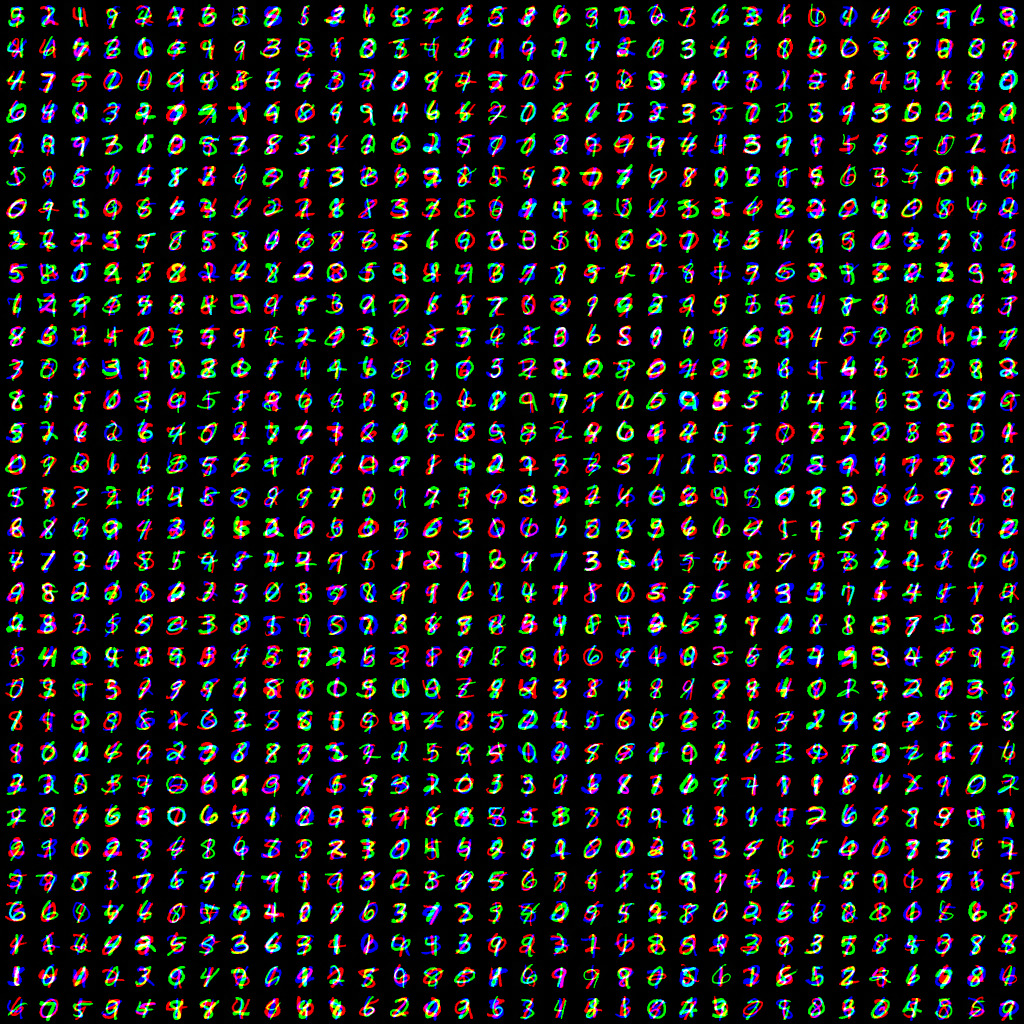
\includegraphics[width=\linewidth, clip, trim={0 0 768px 768px}]{figures/qualitative/stacked-mnist-000008806.jpg}
    \caption{Qualitative examples of sample generation from our Config E on Stacked-MNIST.}
    \label{fig:stacked-mnist}
\end{figure}
}
{
\begin{figure}[ht!]
    %\newlength{\imgsize}
    \setlength{\imgsize}{0.125\linewidth} % Adjust this value to change the size of the images
    
    % New command to include images from a specific directory
    \newcommand{\qualitativeimg}[1]{%
        \includegraphics[width=\imgsize]{figures/qualitative/ffhq-256-000139623/image-#1.jpg}%
    }
    
    \setlength{\tabcolsep}{0pt} % Remove spacing between columns
    \renewcommand{\arraystretch}{0} % Remove spacing between rows
    
    \centering
    \begin{tabular}{cccccccc} % Eight columns
        \qualitativeimg{0} & \qualitativeimg{1} & \qualitativeimg{2} & \qualitativeimg{3} & \qualitativeimg{4} & \qualitativeimg{5} & \qualitativeimg{6} & \qualitativeimg{7} \\
        \qualitativeimg{8} & \qualitativeimg{9} & \qualitativeimg{10} & \qualitativeimg{11} & \qualitativeimg{12} & \qualitativeimg{13} & \qualitativeimg{14} & \qualitativeimg{15} \\
        \qualitativeimg{16} & \qualitativeimg{17} & \qualitativeimg{18} & \qualitativeimg{19} & \qualitativeimg{20} & \qualitativeimg{71} & \qualitativeimg{22} & \qualitativeimg{23} \\
        \qualitativeimg{24} & \qualitativeimg{25} & \qualitativeimg{26} & \qualitativeimg{27} & \qualitativeimg{28} & \qualitativeimg{29} & \qualitativeimg{30} & \qualitativeimg{31} \\
        \qualitativeimg{32} & \qualitativeimg{33} & \qualitativeimg{34} & \qualitativeimg{35} & \qualitativeimg{36} & \qualitativeimg{37} & \qualitativeimg{38} & \qualitativeimg{39} \\
        \qualitativeimg{40} & \qualitativeimg{41} & \qualitativeimg{42} & \qualitativeimg{43} & \qualitativeimg{44} & \qualitativeimg{45} & \qualitativeimg{46} & \qualitativeimg{47} \\
        \qualitativeimg{48} & \qualitativeimg{49} & \qualitativeimg{50} & \qualitativeimg{51} & \qualitativeimg{52} & \qualitativeimg{53} & \qualitativeimg{54} & \qualitativeimg{55} \\
        \qualitativeimg{56} & \qualitativeimg{57} & \qualitativeimg{58} & \qualitativeimg{59} & \qualitativeimg{60} & \qualitativeimg{61} & \qualitativeimg{62} & \qualitativeimg{63} \\
    \end{tabular}
    \caption{More qualitative examples of sample generation from our Config E on FFHQ-256.}
    \label{fig:ffhq-256}
\end{figure}
}
{
% Variable to control the size of each image
\begin{figure}[h!]
%    \newlength{\imgsize}
    \setlength{\imgsize}{0.2\linewidth} % Adjust this value to change the size of the images
    
    \setlength{\tabcolsep}{0pt} % Remove spacing between columns
    \renewcommand{\arraystretch}{0} % Remove spacing between rows

    % New command to include images from a specific directory
    % \newcommand{\qualitativeimg}[1]{%
    %     \includegraphics[width=\imgsize]{figures/qualitative/stacked-mnist-000008806/number-#1.jpg}%
    % }
    \centering
    
    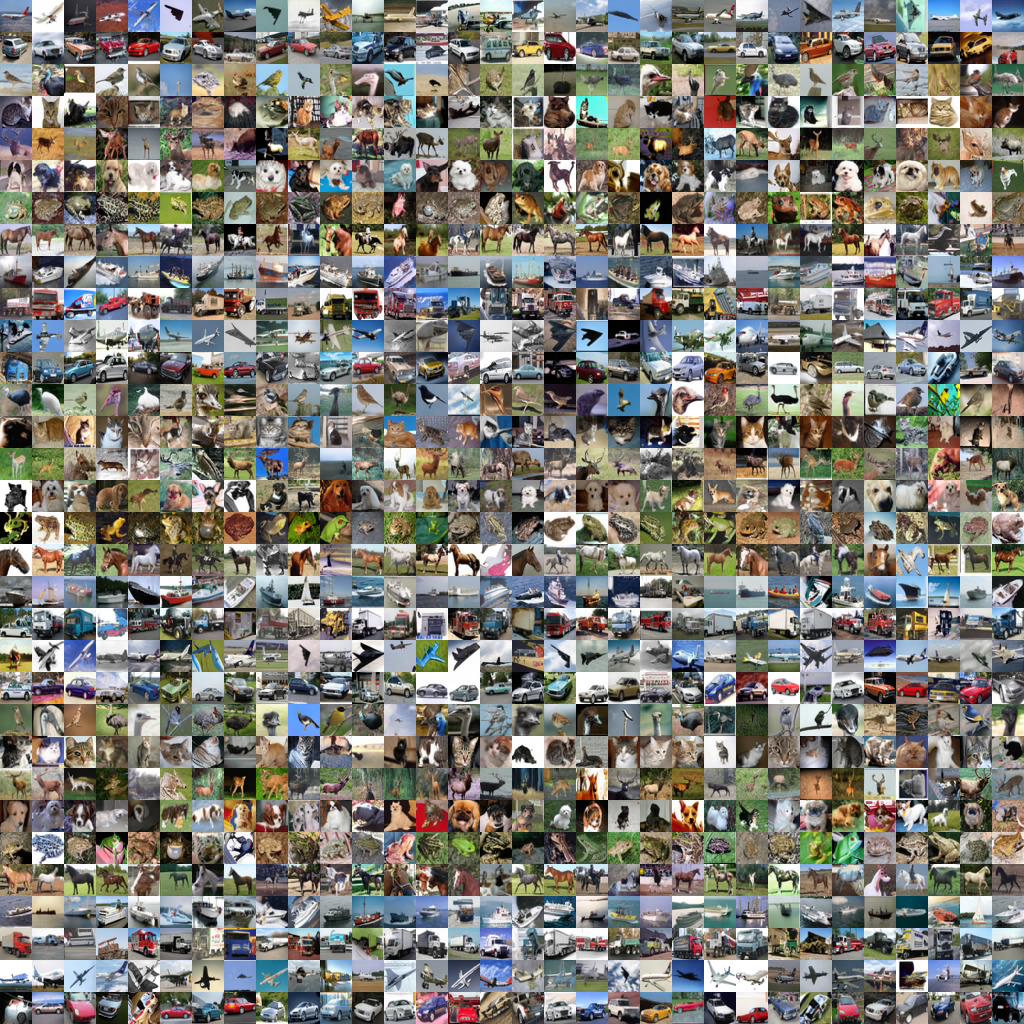
\includegraphics[width=\linewidth]{figures/qualitative/cifar-10-000222209.jpg}
    \caption{Qualitative examples of sample generation from our Config E on CIFAR-10.}
    \label{fig:cifar10}
\end{figure}
}
{
% Variable to control the size of each image
\begin{figure}[ht!]
    %\newlength{\imgsize}
    \setlength{\imgsize}{0.2\linewidth} % Adjust this value to change the size of the images
    
    \setlength{\tabcolsep}{0pt} % Remove spacing between columns
    \renewcommand{\arraystretch}{0} % Remove spacing between rows

    % New command to include images from a specific directory
    \newcommand{\qualitativeimg}[1]{%
        \includegraphics[width=\imgsize]{figures/qualitative/stacked-mnist-000008806/number-#1.jpg}%
    }
    \centering
    
    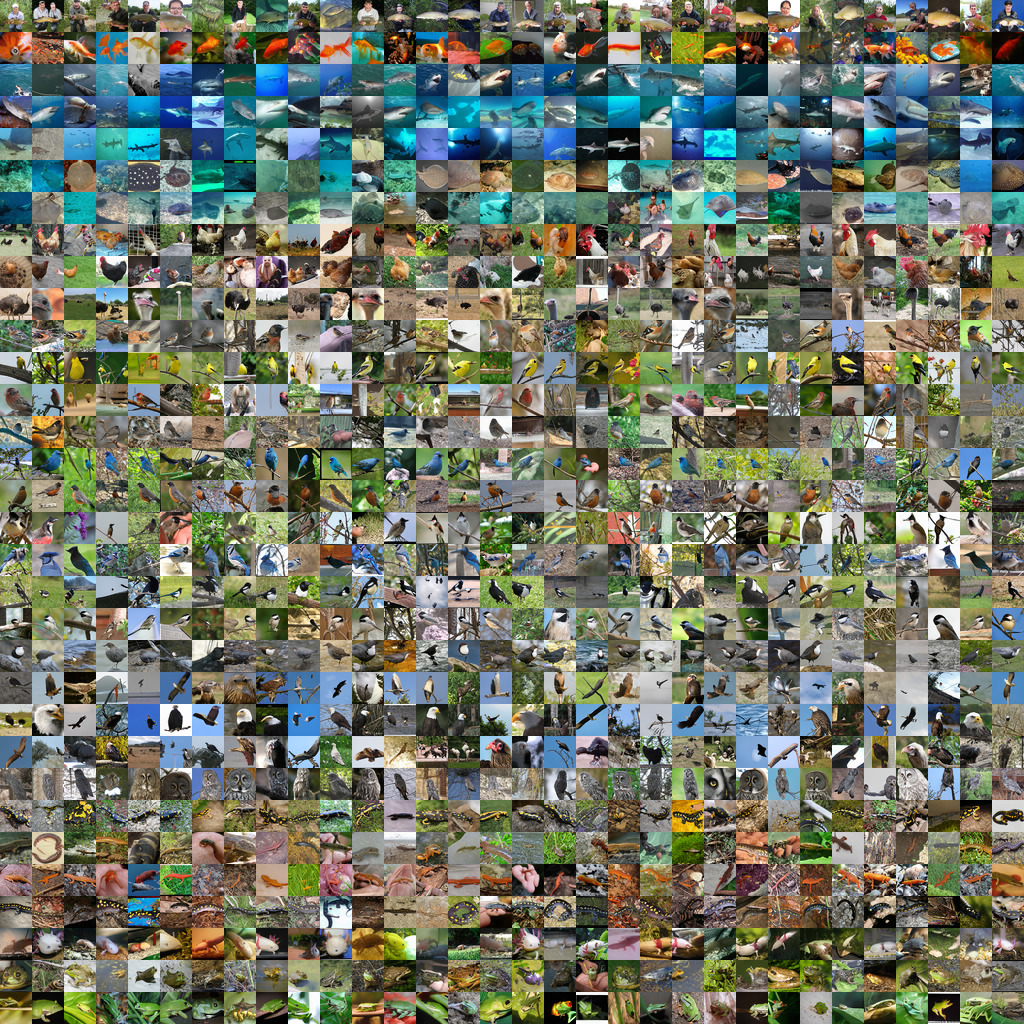
\includegraphics[width=\linewidth]{figures/qualitative/imgnet-32-000681275.jpg}
    \caption{Qualitative examples of sample generation from our Config E on ImageNet-32.}
    \label{fig:imgnet-32}
\end{figure}
}